\documentclass[12pt, a4paper]{article}


\usepackage[top=1.5cm, left=1.5cm, bottom=1.5cm, right=1.5cm]{geometry}
\usepackage{graphicx}

\usepackage[utf8]{inputenc}
\usepackage[T1]{fontenc}
\usepackage[francais]{babel}


\begin{document}
    
    \begin{titlepage}
        \begin{minipage}{.4\linewidth}
            
\includegraphics{img/logo.png}
        \end{minipage}
        \hfill
        \begin{minipage}{.4\linewidth}
            \begin{flushright}
                2017-2018
            \end{flushright}
        \end{minipage}
        
        \vspace{7cm}
        
        \begin{center}
            \textbf{\Huge{Rapport d'expérimentation sur la dynamique des automates cellulaires}}
        \end{center}
        
        \vspace{10cm}
        
        \begin{minipage}{.4\linewidth}
            CASTEL Flavien 21405613\\
            VOISIN Dan 21502515
        \end{minipage}
        \hfill
        \begin{minipage}{.4\linewidth}
            \begin{flushright}
                L2 Informatique
            \end{flushright}
        \end{minipage}
    
    \end{titlepage}
    
    
    \section{Premières évolutions de l'automate de Greenberg-Hastings}
        Sur le premier modèle de Greenberg-Hasting avec un automate cellulaire à trois états et d'une taille 80$\times$80 cases, l'évolution de cet automate ressemble aux figures suivantes:
        \begin{center}
            \begin{figure}[!h]
                \centering
                \begin{minipage}{.3\linewidth}
                    \centering
                    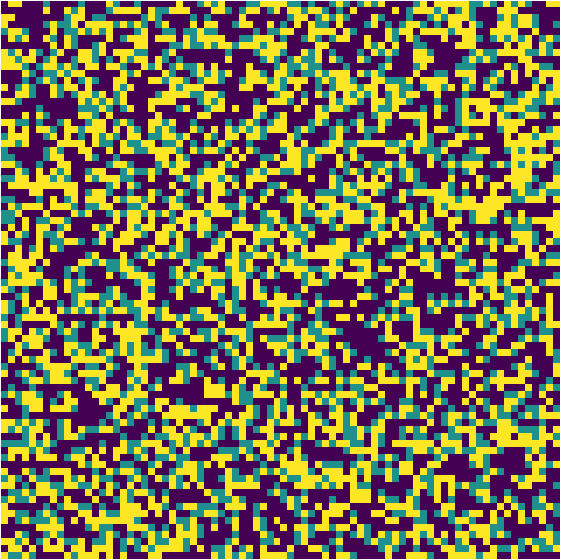
\includegraphics[scale=0.2]{img/step1.png}
                    \caption{Étape 1}
                \end{minipage}
                $\rightarrow$
                \begin{minipage}{.3\linewidth}
                    \centering
                    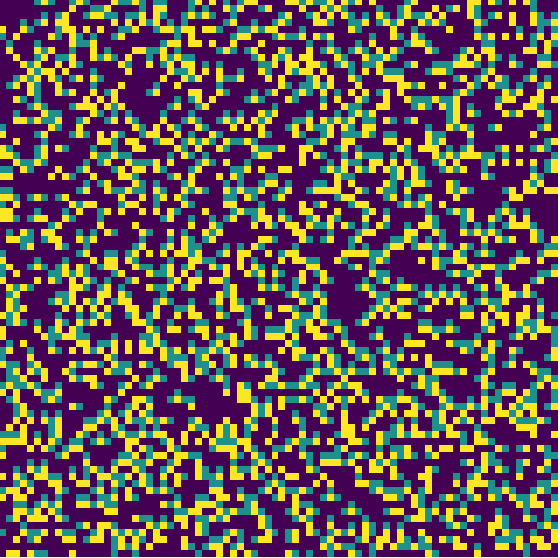
\includegraphics[scale=0.2]{img/step2.png}
                    \caption{Étape 2}
                \end{minipage}
                $\rightarrow$
                \begin{minipage}{.3\linewidth}
                    \centering
                    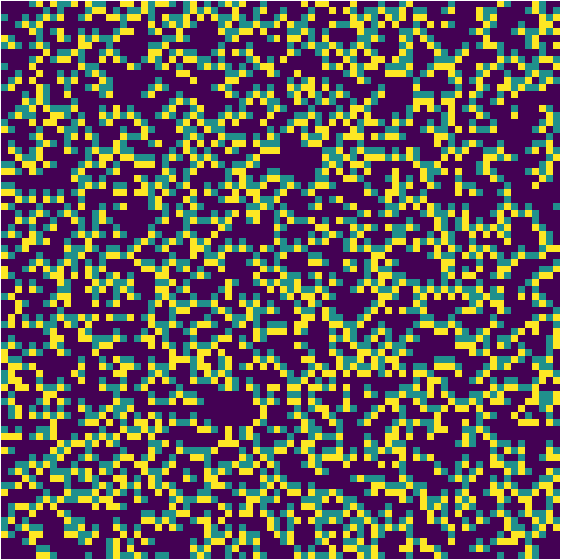
\includegraphics[scale=0.2]{img/step3.png}
                    \caption{Étape 3}
                \end{minipage}
            \end{figure}
            % 2nd line
            \begin{figure}[!h]
                \centering
                $\rightarrow$
                \begin{minipage}{.3\linewidth}
                    \centering
                    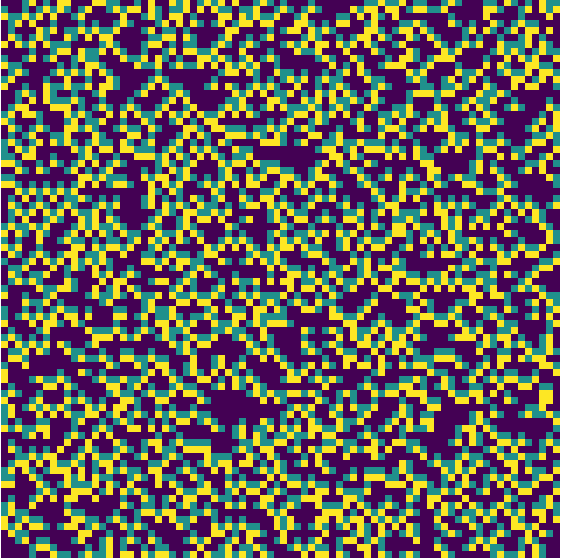
\includegraphics[scale=0.2]{img/step4.png}
                    \caption{Étape 4}
                \end{minipage}
                $\rightarrow$
                \begin{minipage}{.3\linewidth}
                    \centering
                    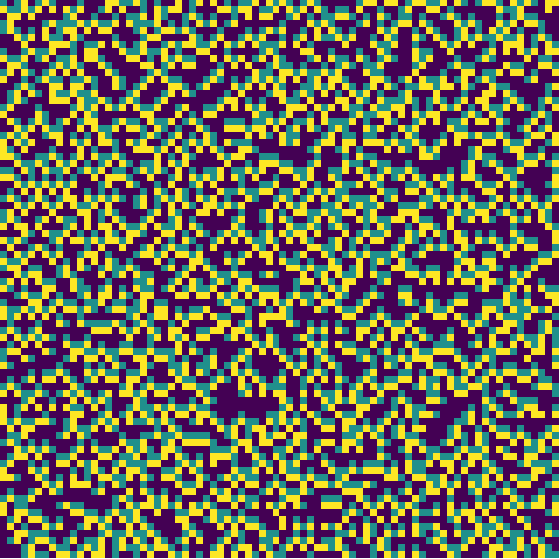
\includegraphics[scale=0.2]{img/step5.png}
                    \caption{Étape 5}
                \end{minipage}
            \end{figure}
        \end{center}
    
    
    \section{Phénomènes d'émergences sur un automate donné}
        \textbf{FAIRE LES IMAGES !!!\\}
        On utilise maintenant un modèle généraliste de Greenberg-Hastings. On utilise comme paramètres huit états possibles par cellules, un rayon de 3 cases, un seuil de 5 et une taille de 80$\times$80.
        \begin{center}
            \begin{figure}[!h]
                \centering
                \begin{minipage}{.3\linewidth}
                    \centering
                    
\includegraphics[scale=0.2]{img/logo.png}
                    \caption{Étape 1}
                \end{minipage}
                $\rightarrow$
                \begin{minipage}{.3\linewidth}
                    \centering
                    
\includegraphics[scale=0.2]{img/logo.png}
                    \caption{Étape 2}
                \end{minipage}
                $\rightarrow$
                \begin{minipage}{.3\linewidth}
                    \centering
                    
\includegraphics[scale=0.2]{img/logo.png}
                    \caption{Étape 3}
                \end{minipage}
            \end{figure}
            % 2nd line
            \begin{figure}[!h]
                \centering
                $\rightarrow$
                \begin{minipage}{.29\linewidth}
                    \centering
                    
\includegraphics[scale=0.2]{img/logo.png}
                    \caption{Étape 4}
                \end{minipage}
                $\rightarrow$
                \begin{minipage}{.3\linewidth}
                    \centering
                    
\includegraphics[scale=0.2]{img/logo.png}
                    \caption{Étape 5}
                \end{minipage}
                $\rightarrow$
                \begin{minipage}{.3\linewidth}
                    \centering
                    
\includegraphics[scale=0.2]{img/logo.png}
                    \caption{Étape 6}
                \end{minipage}
            \end{figure}
        \end{center}
        On remarque que l'automate subit d'abord une phase d'évolution chaotique, puis se stabilise pour répéter le même cycle d'évolution à l'infini.
    
    
    \section{Proposition d'automates créant des phénomènes d'émergeances}
        \textbf{En faisant varier les paramètres nbEtats , rayon , seuil et tail , proposer d'autres automates dont la dynamique présente également des phénomènes d'émergence.\\
        Faire des test\\
        Afficher les images avec les parametres}
    
\end{document}